\documentclass[tikz,border=4pt]{standalone}
\usepackage{amsmath}
\usepackage{graphicx}
\usepackage{tikz}
\usetikzlibrary{calc}

\newcommand{\marTwentySixFormulaFont}{\fontsize{8}{8}\selectfont}
\newcommand{\marTwentySixNumberFont}{\fontsize{12}{12}\selectfont}

\tikzset{
  mar26 formula/.style={font=\marTwentySixFormulaFont,text=black,anchor=center,inner sep=0pt,outer sep=0pt},
  mar26 psi/.style={font=\marTwentySixFormulaFont,text=black,anchor=center,inner sep=0pt,outer sep=0pt},
  mar26 phi/.style={font=\marTwentySixFormulaFont,text=black,anchor=center,inner sep=0pt,outer sep=0pt},
  mar26 plus/.style={font=\marTwentySixFormulaFont,text=black,anchor=center,inner sep=0pt,outer sep=0pt},
  mar26 equals/.style={font=\marTwentySixFormulaFont,text=black,anchor=center,inner sep=0pt,outer sep=0pt},
  mar26 pair title/.style={font=\marTwentySixFormulaFont,text=black,anchor=center,inner sep=0pt,outer sep=0pt},
  mar26 pair data/.style={font=\marTwentySixFormulaFont,text=black,anchor=center,inner sep=0pt,outer sep=0pt},
  mar26 number/.style={font=\marTwentySixNumberFont,text=black,anchor=center,inner sep=0pt,outer sep=0pt,text height=1.5ex,text depth=0.25ex},
  mar26 neighbour number/.style={font=\marTwentySixNumberFont,text={rgb,1:red,0.55;green,0.55;blue,0.55},anchor=center,inner sep=0pt,outer sep=0pt,text height=1.5ex,text depth=0.25ex}
}

\begin{document}
\begin{tikzpicture}
  \node[inner sep=0pt,outer sep=0pt] (img) at (0,0) {%
    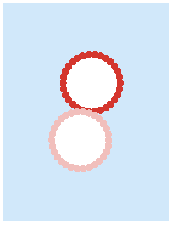
\includegraphics{mar26_visualse_coarse_fine_new_rotation_fig6.pdf}%
  };
  % Auto-generated from mar26_visualse_coarse_fine_new_rotation.m
\begin{scope}[shift={(img.south west)},
  x={($(img.south east)-(img.south west)$)},
  y={($(img.north west)-(img.south west)$)}]
  \node[mar26 number] at (0.5000013199504652, 1.0046928445607266) {};
  \node[mar26 number] at (0.5000013199504652, 1.0046928445607266) {};
  \node[mar26 pair data] at (0.5000000000000000, 0.8355154944404237) {$\mathbf{u} = \mathbf{0}$};
  \node[mar26 formula] at (0.5344747323229710, 0.6315547075465491) {$i$};
  \node[mar26 formula] at (0.4655252676770290, 0.3684452924534509) {$j$};
  \node[mar26 pair title] at (0.1982620390006724, 0.5789196657674848) {$\boldsymbol{\eta}^{(i,j)}$};
  \node[mar26 pair data] at (0.6896670632252280, 0.2105401671162577) {$\mathbf{u} = -\boldsymbol{\phi}^{(i)}$};
\end{scope}

\end{tikzpicture}
\end{document}
